\documentclass{beamer}

%%%%%%%%%%%%%Solarized Theme%%%%%%%%%%%%%%%
\usecolortheme[dark,accent=cyan]{solarized}
\beamertemplatenavigationsymbolsempty
%%%%%Packages%%%%%
\usefonttheme{serif}

% \usepackage{fontspec}
% \setmainfont{Helvetica Neue}

\usepackage{graphicx}
\usepackage{hyperref}
\usepackage{colortbl, xcolor}
\usepackage{booktabs}
\usepackage{amsmath,amsthm, amssymb, latexsym}

\usepackage{tikz}
\usepackage{standalone}
\usetikzlibrary{calc, positioning, arrows, arrows.meta, shapes}

\begin{document}

\begin{frame}
    \begin{center}
        \Large{\textcolor{orange}{Stability of defection, optimisation of
        strategies and testing for extortion in the Prisoner's Dilemma}} \\

        \vspace{1.5cm}
        \normalsize{Nikoleta E. Glynatsi}

        \vspace{1cm}
        \small{Dr Vincent Knight} \hspace{4mm} \small{Dr Jonathan Gillard} \hspace{4mm} \small{Dr Marc Harper}

    \end{center}
\end{frame}

\begin{frame}
    \begin{center}
    
\includegraphics[width=0.24\textwidth]{static/cardiff_uni_logo.jpg}\hspace{10pt}
    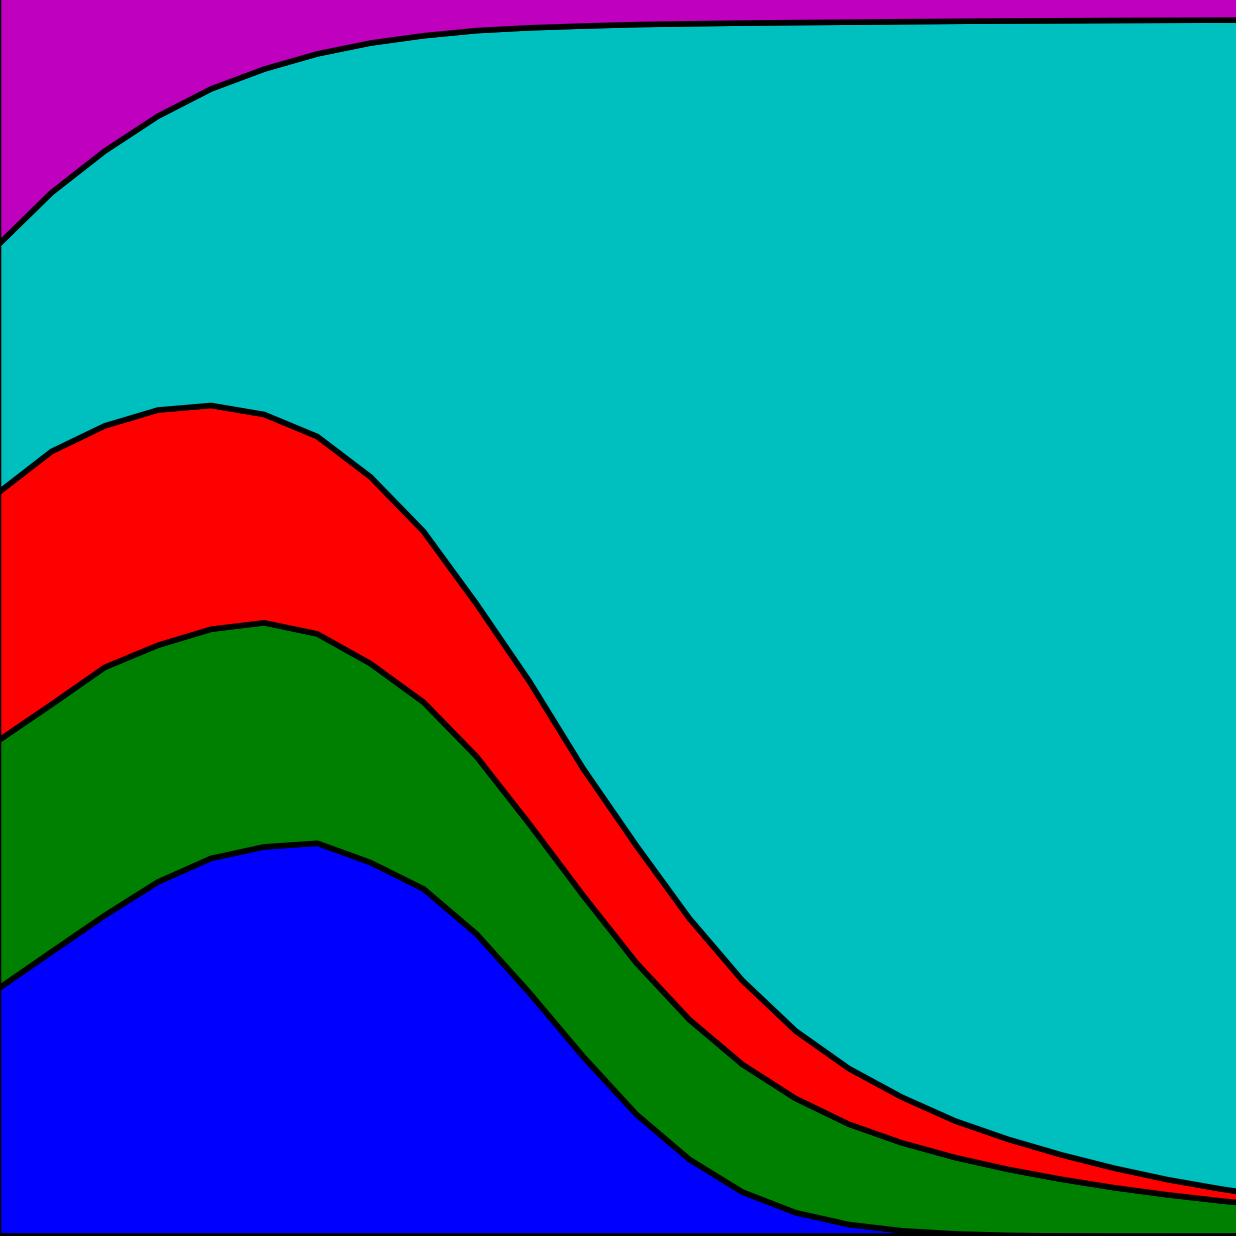
\includegraphics[width=0.24\textwidth]{static/axelrod-logo.png}\vspace{10pt}

    
\includegraphics[width=0.24\textwidth]{static/ssi-logo.png} \hspace{10pt}
    
\includegraphics[width=0.24\textwidth]{static/plos-logo.jpg}
    \vspace{10pt}
    \end{center}
\end{frame}

\begin{frame}
        \includestandalone[width=.9\textwidth]{static/pd}
\end{frame}

\begin{frame}
\Huge{
$$S_p = \begin{pmatrix} 3 & 0  \\ 5 & 1 \end{pmatrix} \quad S_q =
\begin{pmatrix} 3 & 5 \\ 0 & 1 \end{pmatrix}$$}
\end{frame}

\begin{frame}
    \begin{center}
        \normalsize{Effective Choice in the Prisoner's Dilemma - Robert Axelrod, 1980}

        \vspace{.8cm}
        \hspace{-.3cm}\includestandalone[width=.45\textwidth]{static/axelrods_tournament}
    \end{center}
\end{frame}

\begin{frame}
    \begin{center}
        \vspace{-.51cm}
        \normalsize{Iterated Prisoner's Dilemma contains strategies that dominate any evolutionary opponent - William H. Press and Freeman J. Dyson, 2012}

        \vspace{1cm}
        \includestandalone[width=.9\textwidth]{static/extortionate}
    \end{center}
\end{frame}

\begin{frame}
    \begin{center}
        \vspace{.5cm}

        \normalsize{Recognising and evaluating the effectiveness of extortion in
        the Iterated Prisoner's Dilemma - Vincent A. Knight, Marc Harper,
        Nikoleta E. Glynatsi and Jonathan Gillard, 2019}

        \vspace{1.5cm}
        \includestandalone[width=.9\textwidth]{static/sse_method}
    \end{center}
\end{frame}

\begin{frame}
    \begin{center}
        \vspace{1cm}

        \normalsize{Extortion and cooperation in the Prisoner's Dilemma -
        A. J. Stewart and J. B. Plotkin., 2012}

        \vspace{.5cm}
        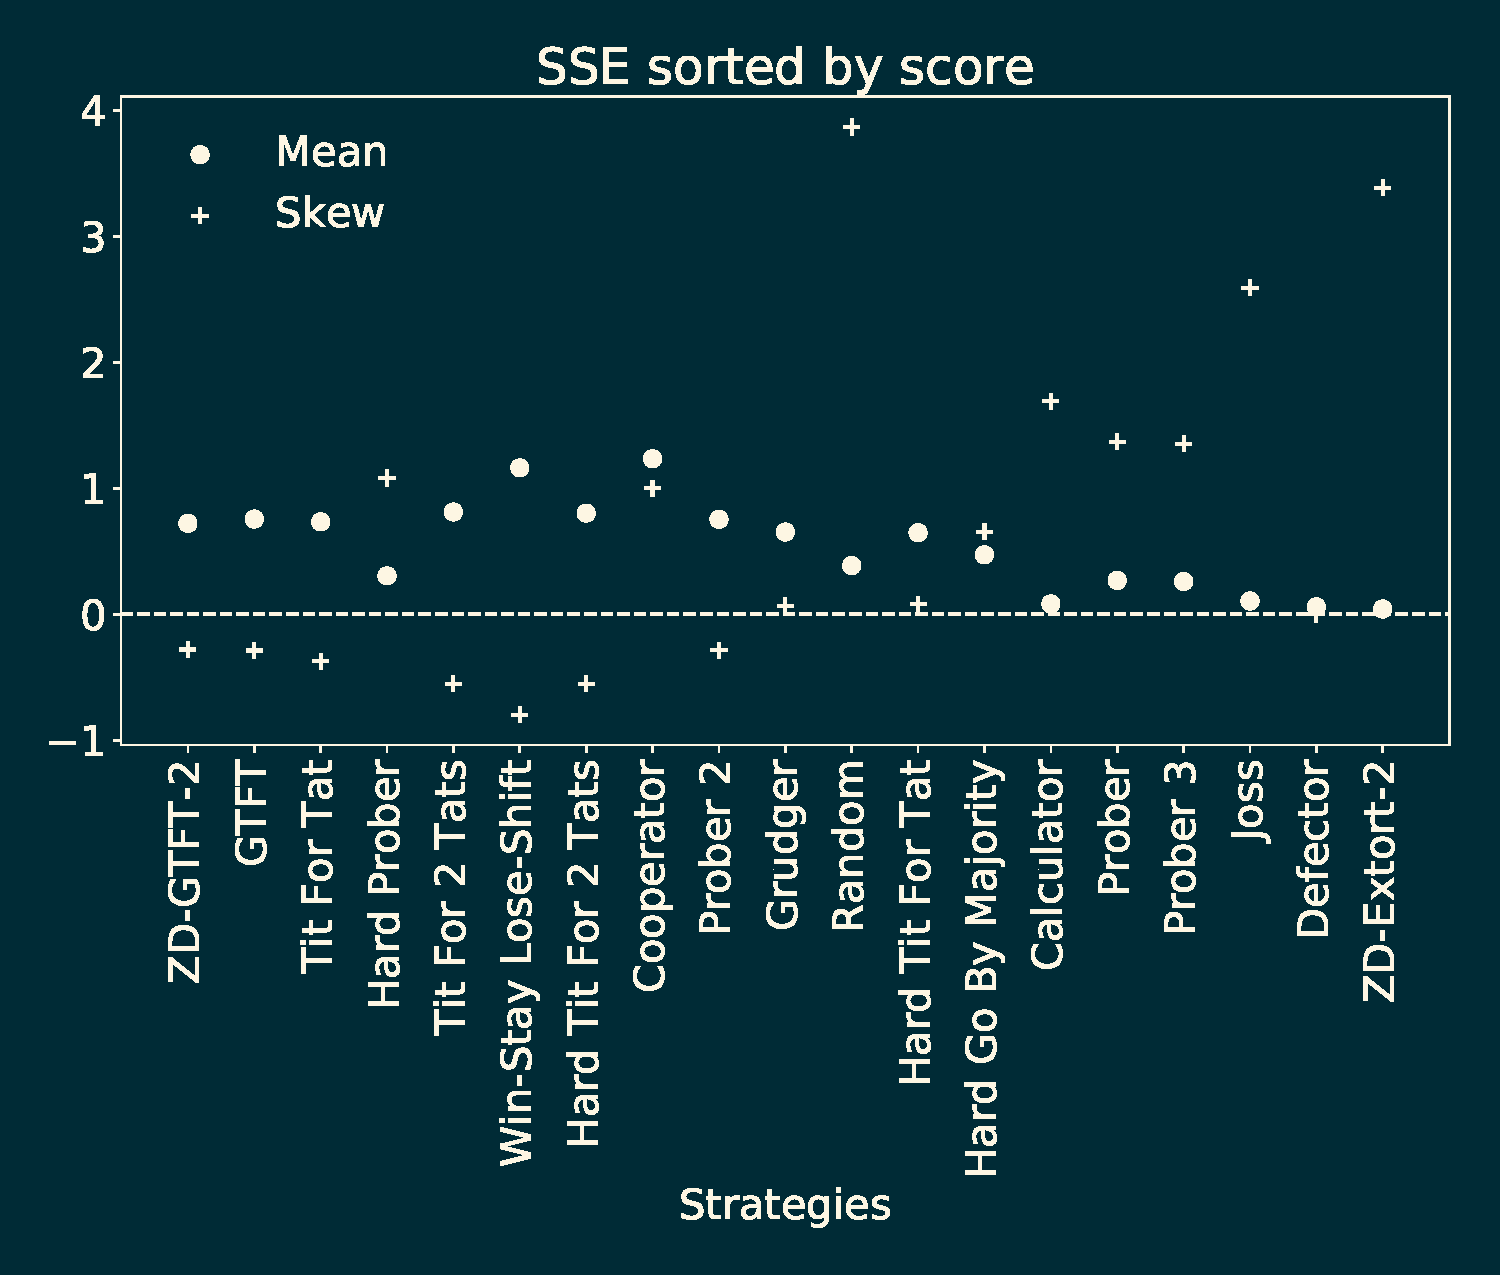
\includegraphics[width=.7\textwidth]{static/validation_plot}
    \end{center}
\end{frame}

\begin{frame}
    \begin{center}
        \vspace{-1cm}
        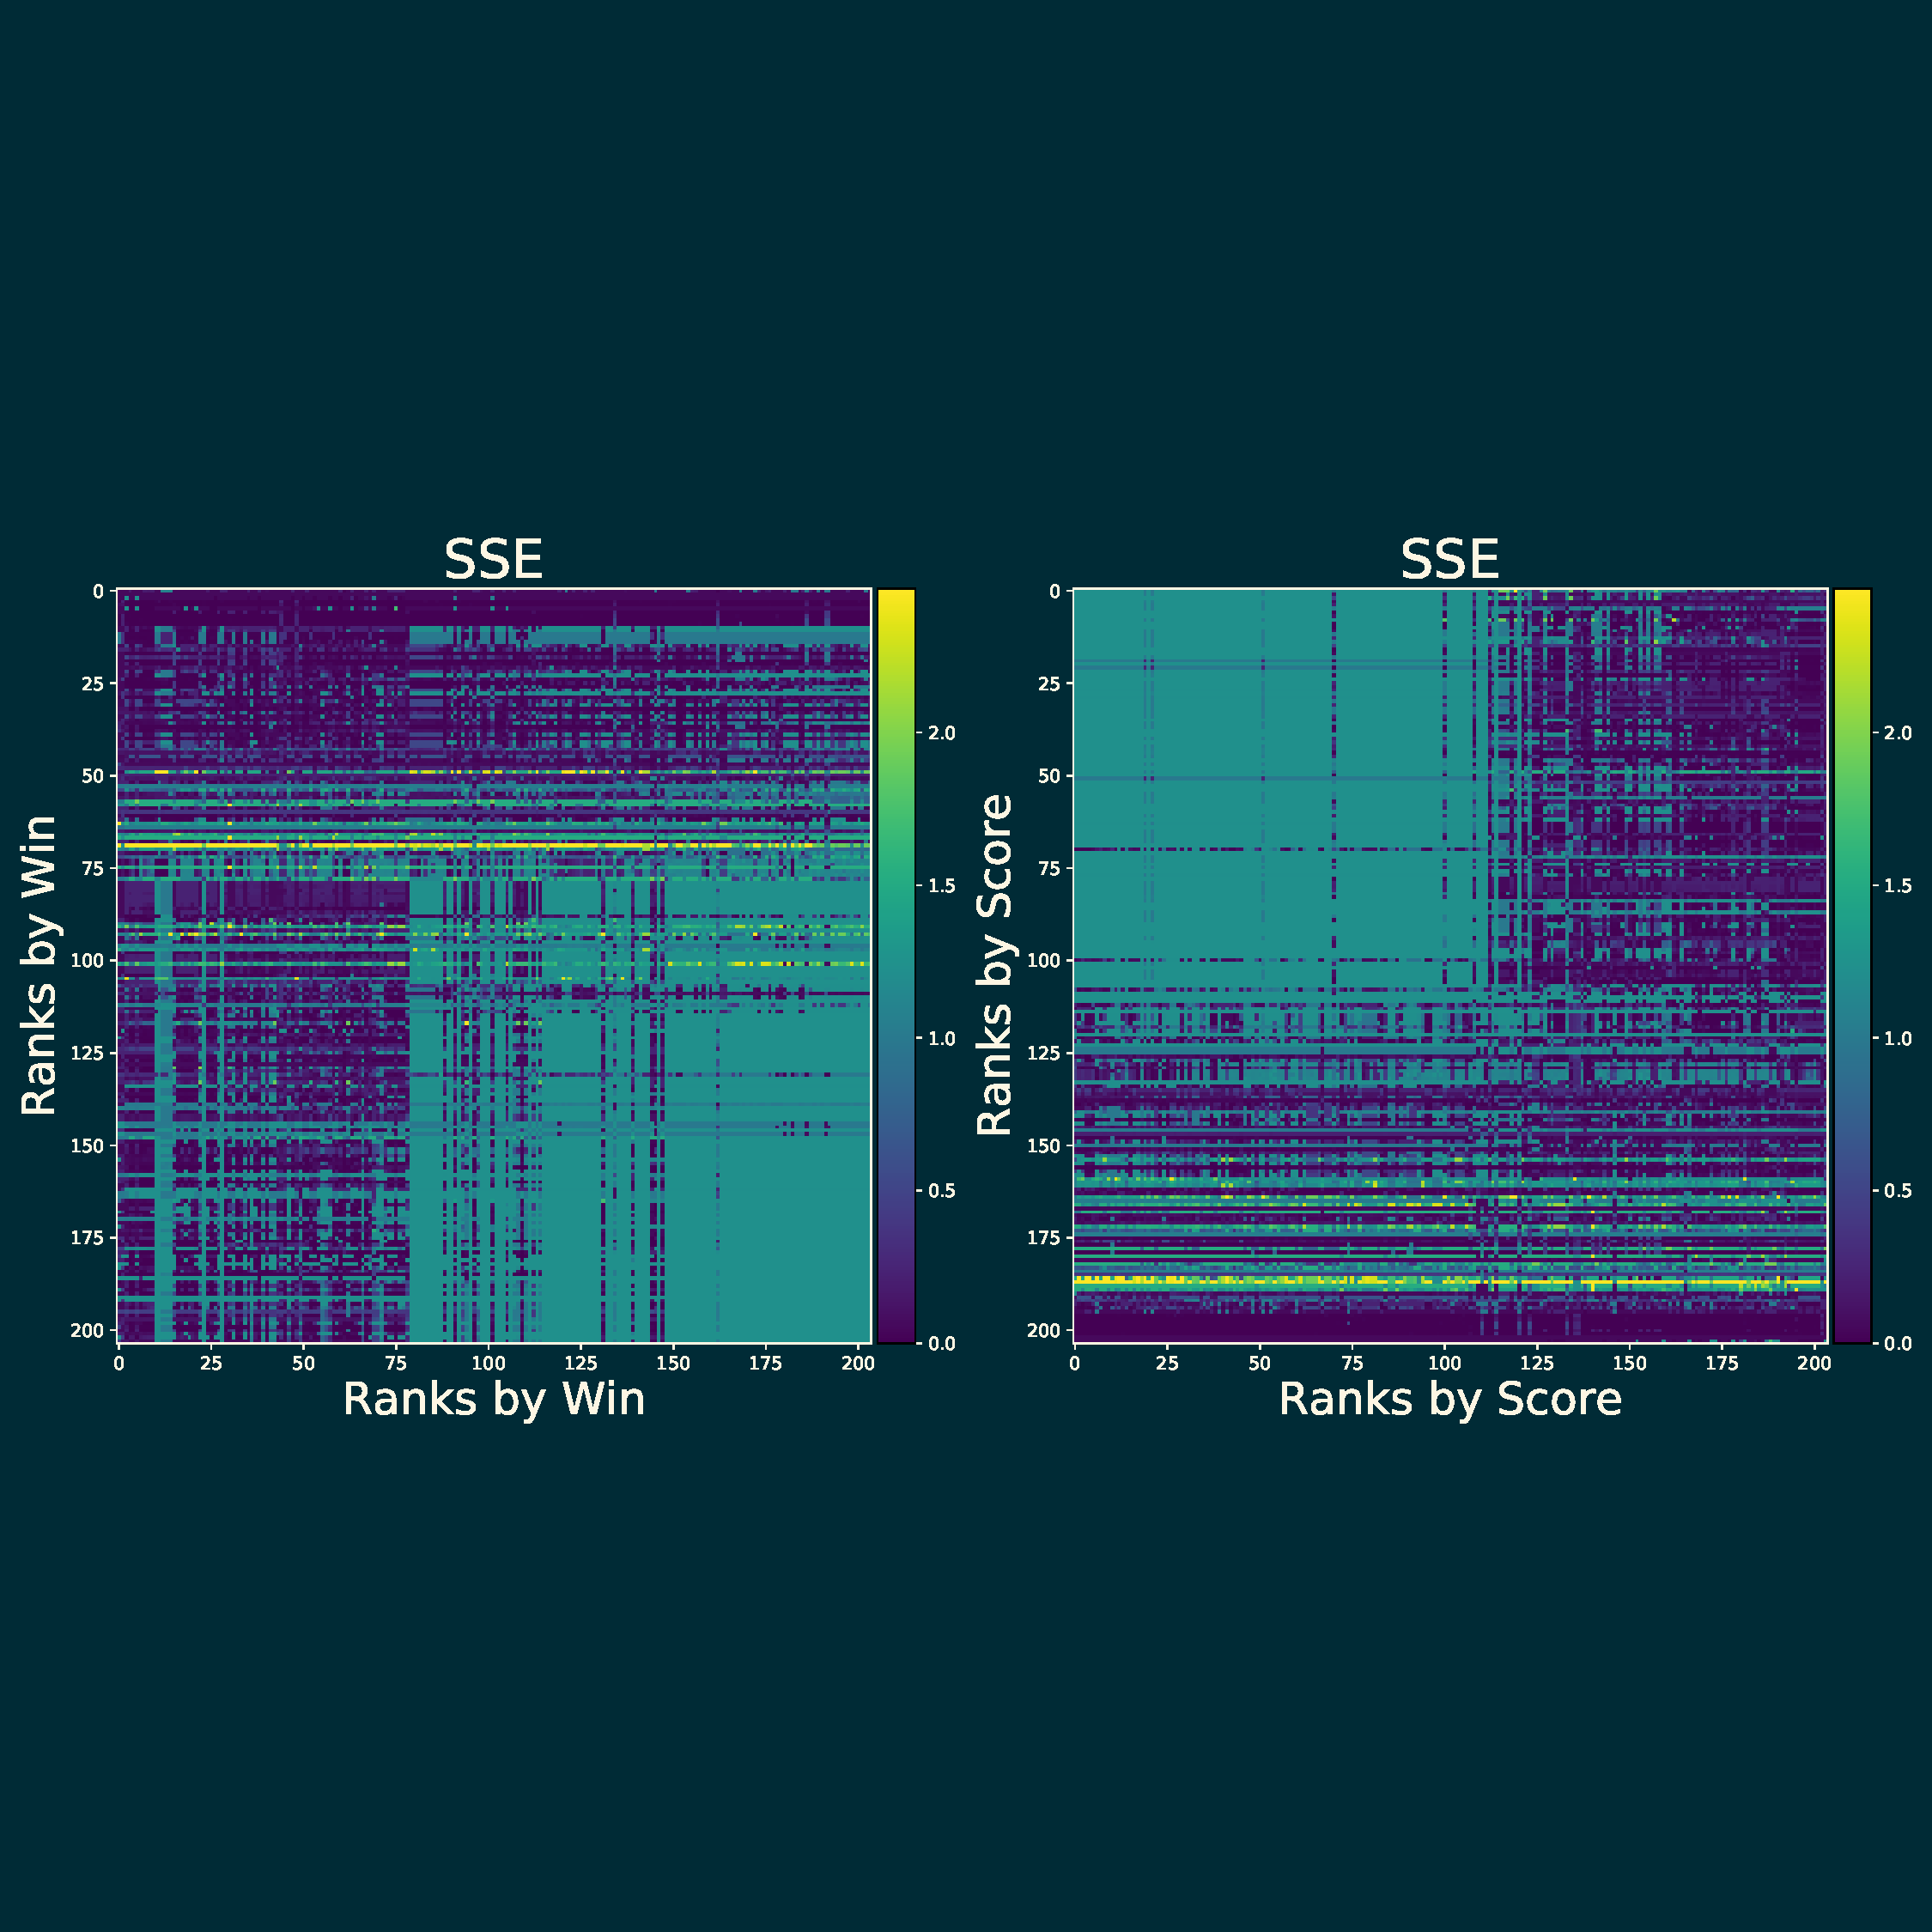
\includegraphics[width=\textwidth]{static/results_sserror}
    \end{center}
\end{frame}

\begin{frame}
    \begin{center}

        \normalsize{Stability of defection, optimisation of strategies and th
        limits of memory in the Prisoner's Dilemma - Nikoleta E. Glynatsi and
        Dr Vincent Knight}
        
        \vspace{.5cm}
        \includestandalone[width=\textwidth]{static/best_responses}
    \end{center}
\end{frame}

\begin{frame}
    \begin{center}
        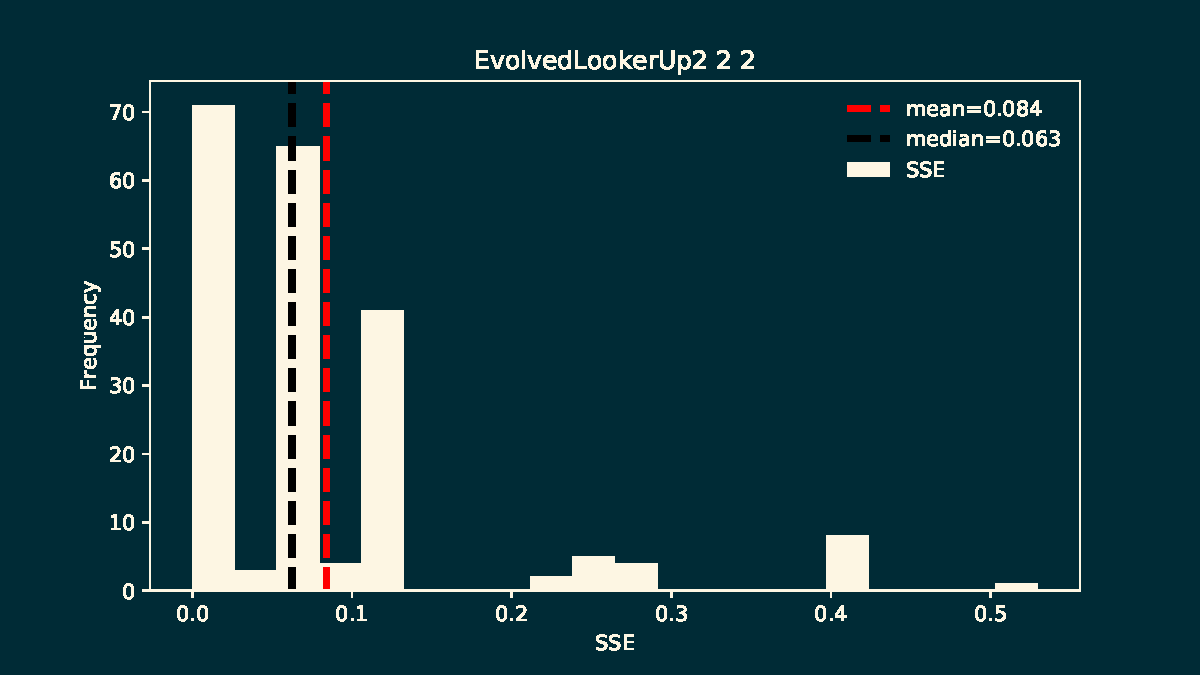
\includegraphics[width=\textwidth]{static/sse_top_strategy}
    \end{center}
\end{frame}

\begin{frame}
    \begin{center}
        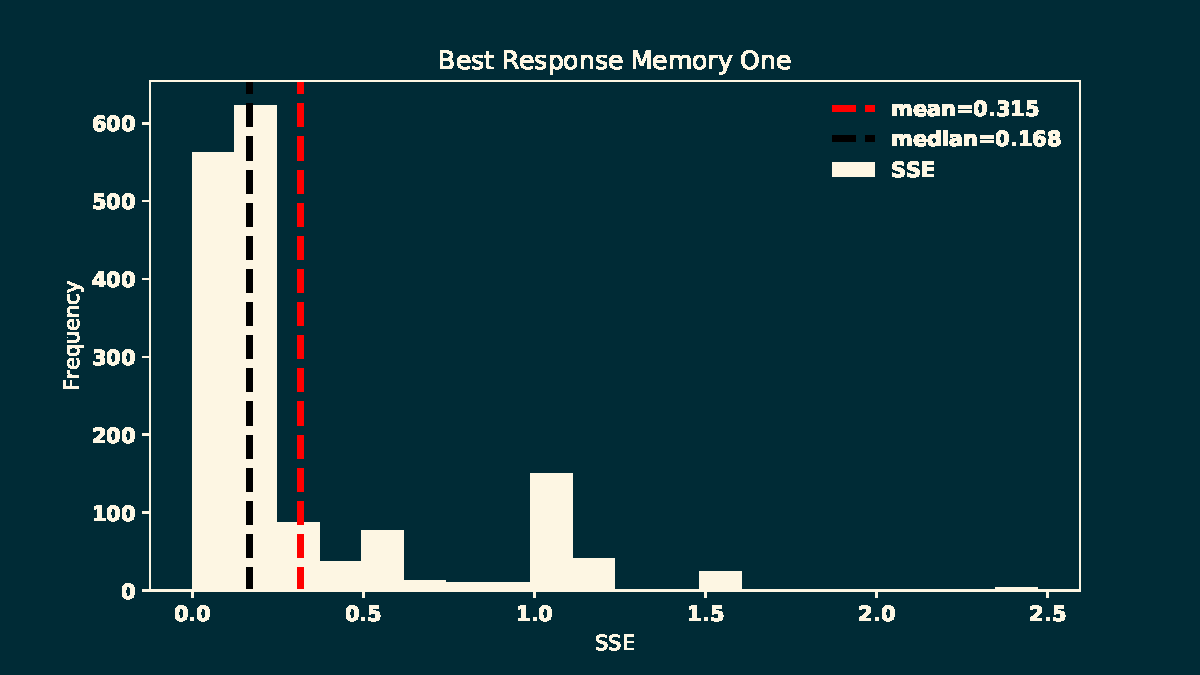
\includegraphics[width=\textwidth]{static/result_best_response}
    \end{center}
\end{frame}

\begin{frame}
    \begin{center}
        \hspace{-2cm}
        \includestandalone[width=.9\textwidth]{static/evolution}
    \end{center}
\end{frame}

\begin{frame}
    \begin{center}
        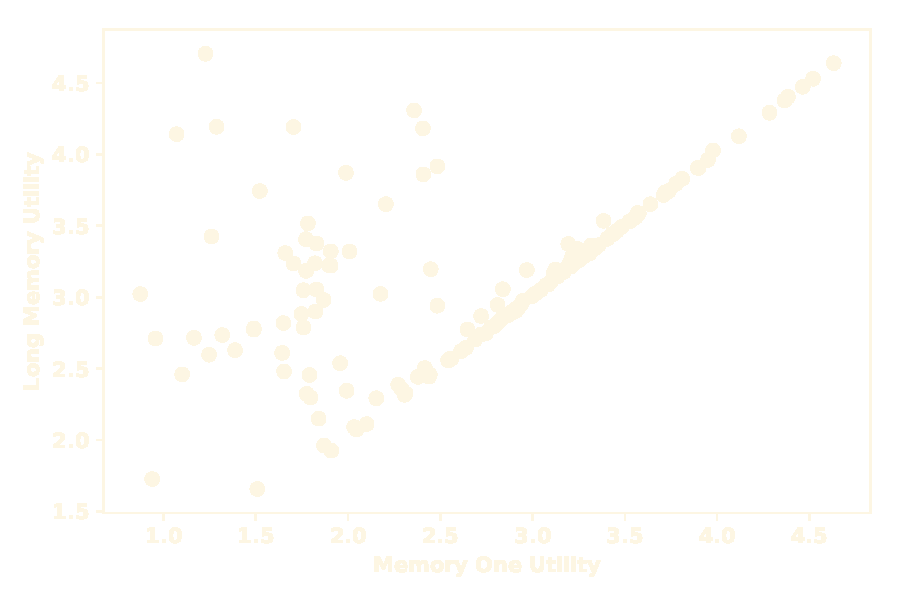
\includegraphics[width=\textwidth]{static/result_gambler}
    \end{center}
\end{frame}

\begin{frame}
    \begin{center}

        \hspace{-.7cm}
        \includestandalone[width=\textwidth]{static/summary}
    \end{center}
\end{frame}

\begin{frame}
    \centering
    
\includegraphics[width=.8\textwidth]{static/tweet}

    \vspace{.4cm}
    @NikoletaGlyn  \\ Glynatsine@cardiff.ac.uk \\

    \vspace{.3cm}
    \small{https://arxiv.org/abs/1904.00973}
\end{frame}

\begin{frame}
    \begin{center}
        \vspace{-1cm}
        \normalsize{Stability of defection, optimisation of strategies and th
        limits of memory in the Prisoner's Dilemma - Nikoleta E. Glynatsi and
        Dr Vincent Knight}

        \vspace{1cm}
        \includestandalone[width=\textwidth]{static/evolutionary_responses}
    \end{center}
\end{frame}

\begin{frame}
    \begin{center}
        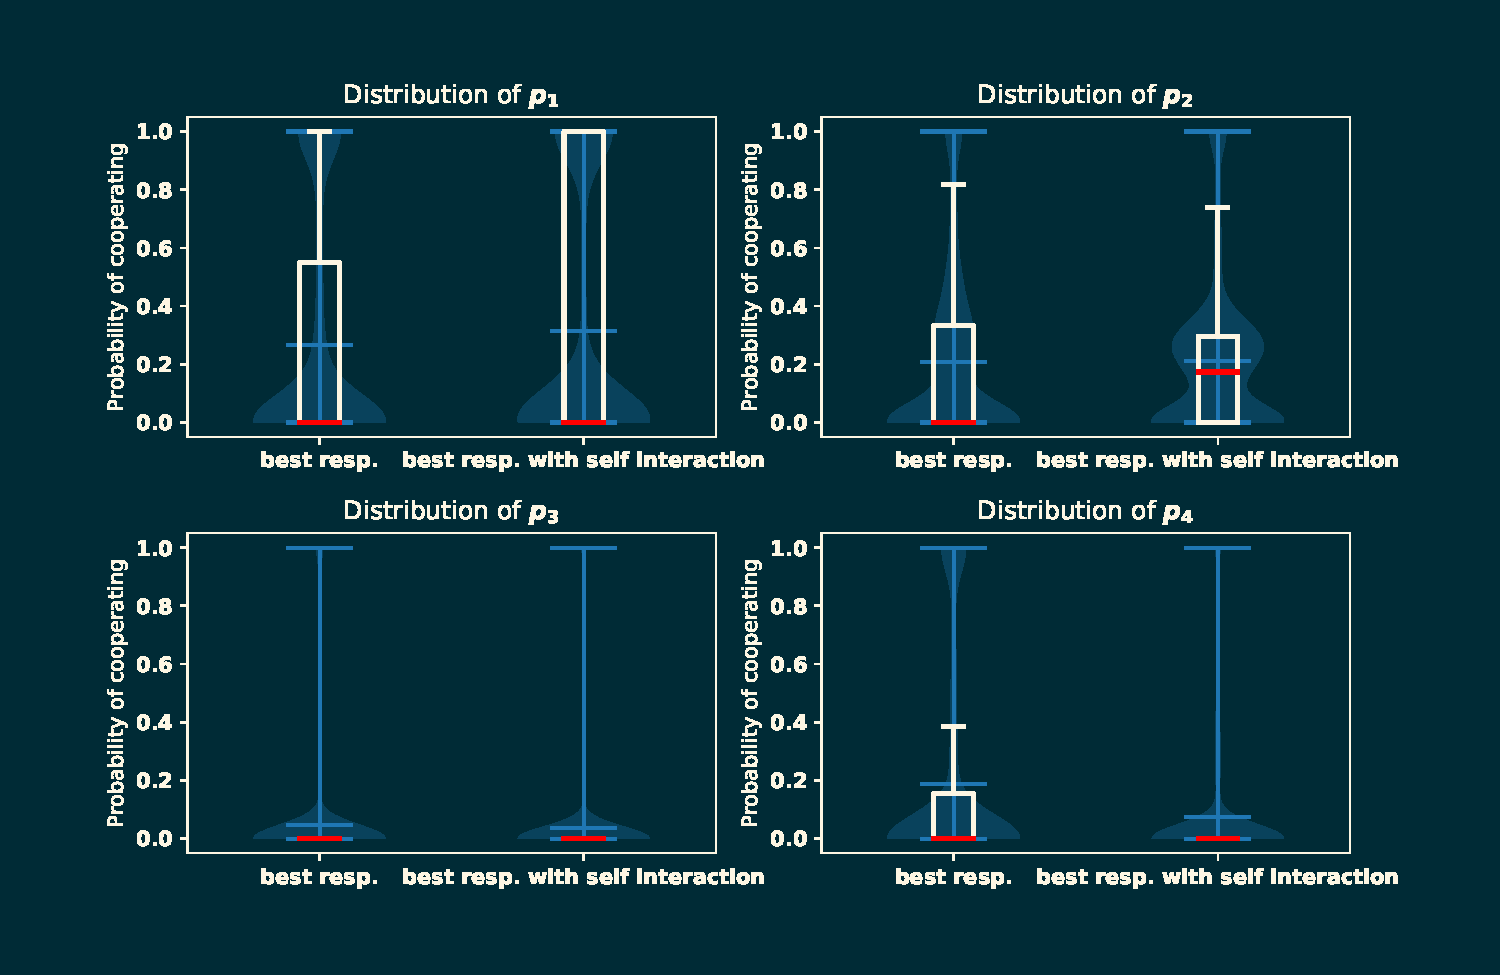
\includegraphics[width=\textwidth]{static/result_self_interactions}
    \end{center}
\end{frame}
\end{document}

